
\documentclass[12pt, a4paper]{report}
\RequirePackage{apacite}
\usepackage{amsfonts,amsmath,amsthm,amssymb,amsopn}
\usepackage{comment}
\usepackage{graphicx}
\usepackage{apacite}

\usepackage[utf8x]{inputenc}
\usepackage{ucs}
\usepackage{listings}
\usepackage{apacite}
\usepackage{multirow}
\usepackage{natbib}
\usepackage{url}

\usepackage{fancyvrb}
\usepackage{color}
%\usepackage[ascii]{inputenc}


%----------------------------------------------------------------------------------------------
 \pagestyle{plain}
 \linespread{1.37}
 \textwidth=14.5cm
 \textheight=22cm
%----------------------------------------------------------------------------------------------

% --- NEW COMMANDS ---
 \newcommand{\C}{{\mathbb C}}
 \newcommand{\Q}{{\mathbb Q}}
 \newcommand{\Z}{{\mathbb Z}}
 \newcommand{\R}{{\mathbb R}}
 \newcommand{\N}{{\mathbb N}}
 \newcommand{\PP}{{\mathbb P}}
 \newcommand{\A}{{\mathbb A}}
 \newcommand{\F}{{\mathbb F}}
 \newcommand{\hash}{\#}
 \newcommand{\divides}{\mid}
 \newcommand{\notdivides}{\nmid}
 \newcommand{\maxdivides}{\parallel}
 \newcommand{\nequiv}{\not \equiv}

%----------------------------------------------------------------------------------------------
 % --- NEW THEOREMS ---
 \newtheorem{thm}{Theorem}[section]
 \newtheorem{lem}[thm]{Lemma}
 \newtheorem{cor}[thm]{Corollary}
 \newtheorem{conj}[thm]{Conjecture}

\newenvironment{defn}{\trivlist \item [\hskip
\labelsep {\bf Definition:}]\ignorespaces}{\endtrivlist}
\newenvironment{rem}{\trivlist \item [\hskip
\labelsep {\bf Remark:}]\ignorespaces}{\endtrivlist}
\newenvironment{rems}{\trivlist \item [\hskip
\labelsep {\bf Remarks:}]\ignorespaces}{\endtrivlist}
\newenvironment{example}{\trivlist \item [\hskip
\labelsep {\bf Example:}]\ignorespaces}{\endtrivlist}
\newenvironment{prf}{\trivlist \item [\hskip
\labelsep {\bf Proof:}]\ignorespaces}{\endtrivlist}

\begin{document}

\parindent=1cm
\thispagestyle{empty}
%
%\pagenumbering{roman} \thispagestyle{empty}

\vspace*{40mm}

\begin{center}

{\LARGE \sc Differential Cryptanalysis of Block Ciphers}

\vspace{20mm}

{\Large Matthew Laten}

\vspace{10mm}

Third Year Maths Project

Supervisor: Dr Christine Swart

\end{center}


\newpage


\vspace*{3cm}

\begin{center}
``Two can keep a secret if one is dead..." - Anon
\begin{comment}
No one has yet discovered any warlike purpose to be served by the
theory of numbers...and it seems very unlikely that anyone will do
so for many years.

G.H. Hardy, 1940.
\end{comment}
\end{center}

%\newpage
%\section*{No Plagiarism Declaration\\}
\Large{\textbf{Final Mathematics Project 2012}\\}
\large{\textbf{Declaration by student:}}
\begin{itemize}
\item I know that plagiarism is wrong. Plagiarism is to use another's work and to pretend that it is one's own.
\item Each significant contribution to, and quotation in, this project from the work of other people has been attributed, and has been cited and referenced.
\item This report is my own work.
\item I have not allowed, and will not allow, anyone to copy my work with the intention of passing it off as his or her own work.\\\\
\end{itemize}
\textbf{Name:} Matthew Laten\\
\textbf{Student Number:} LTNMAT001\\
\textbf{Signature:}\\
\textbf{Date:}\\

\newpage

\begin{center}
\Large \bf Abstract
\end{center}

In this paper we discuss the mathematics behind attacking a Block Cipher by
means of Differential Cryptanalysis. To this end, we lay down some background
knowledge in the fields of Probability Theory, Boolean Algebra and Block
Ciphers themselves first, along with examples and the necessary mathematical
theorems. We then move on to explaining what Differential Cryptanalysis is, how
it works, and how we can use it against Substitution-Permutation Networks. We
conclude with a walkthrough of the process by means of an example. 


\newpage
\tableofcontents
\nocite{king}


%%%%%%%%%%%%%%%%%%%%%%%%%%%%%%%%%%%%%%%%%%%%%%%%%%%%%%%%%%%%%%%%%%%
%                                                                 %
%                       Introduction                              %
%                                                                 %
%%%%%%%%%%%%%%%%%%%%%%%%%%%%%%%%%%%%%%%%%%%%%%%%%%%%%%%%%%%%%%%%%%%


\chapter{Introduction} \label{c:introduction}
Imagine a world without encryption. Anyone with access to a computer could
steal your money, impersonate you, or learn your secrets.  Privacy would be
dead. The inability to secure information might even lead to police states,
where governments will have to resort to desparate measures to protect their
secrets.  Fortunately, we do not live in such a world. We live in a world where
encryption is a very real part of our daily lives. Whether banking online,
shopping for new items or chatting to your friends on your favourite social
network, you are indirectly using various forms of encryption to keep your
messages safe, and indicate to computer servers that you are who you say you
are.

So if our data is all secure and encrypted, why should we worry more about the
subject of Cryptography? In short, our data isn't secure. Attackers find more
and more ingenious ways of breaking implementations and protocols, even when
the encryption method is said to be secure. The premier algorithm for
encrypting electronic data from 1979 onwards, known as the Data Encryption
Standard (DES), was publicly broken in 1997. Today's encryption standards are
tomorrow's broken algorithms. So we, as cryptographers, have the responsibility
to make encryption more secure; even in some cases, to improve the manner in
which these algorithms are implemented!  How can we do this? By doning a black
hat and thinking like an attacker. In this paper, we will be looking at an
attack on block ciphers, specifically known as differential cryptanalysis. But
first, we should probably define some unfamiliar terminology.

\section{Terminology}

\begin{rem}
Note, this paper assumes that you have an adequate knowledge of 3rd year
university level Mathematics, but a knowledge of Cryptography or Probability
theory is not required, as all concepts necessary for understanding this paper
will be explained.
\end{rem}

As you might already know, \textbf{Cryptography} is the discipline concerned
with keeping data secret, or more formally, it is the study and practice of
techniques and algorithms for securing the transference of data in the presence
of third parties, known as attackers or adversaries.  \textbf{Cryptanalysis}
however, deals with the breaking of these techniques and retrieval of the
secret data. 

In cryptography, \textbf{encryption} refers to the process of converting
plaintext, or data that is easily understandable, into ciphertext, that is
unintelligible data. The reverse process of converting the cipher text back
into plaintext is known as \textbf{decryption}. In most cases, this encryption
or decryption occurs with the aid of a \textbf{key}, a parameter that
determines the functional output of the cryptographic algorithm.

Furthermore, there are two main types which come up when discussing key-based
cryptography, namely Symmetric-key, and Asymmetric-key or Public-key
cryptography.  In the case of \textbf{Symmetric-key}, the same key is used for
encryption and decryption, while with \textbf{Asymmetric-key}, a key is made
available to the public for encryption, and only those posessing the secret or
private key will be able to decrypt messages encrypted with the matching public
key.

A \textbf{block cipher} is a type of Symmetric-key encryption cipher that
operates on a fixed-length ``block'' of data. This is in contrast to a
\textbf{stream cipher}, which operates on a potentially infinite stream of
data. For the purposes of this paper, we will define a block cipher in more
depth later, but at the moment we have enough of a vocabulary to delve into a
bit of supporting knowledge.



%%%%%%%%%%%%%%%%%%%%%%%%%%%%%%%%%%%%%%%%%%%%%%%%%%%%%%%%%%%%%%%%%%%
%                                                                 %
%                           Background                            %
%                                                                 %
%%%%%%%%%%%%%%%%%%%%%%%%%%%%%%%%%%%%%%%%%%%%%%%%%%%%%%%%%%%%%%%%%%%


\chapter{Background} \label{c:background}

We will start by looking at some basic Probability Theory, and then move on to
Boolean Algebra. To conclude this section, we will introduce Block Ciphers and
the interesting properties surrounding them. We will only define concepts that
are needed as stepping stones to explaining Differential Cryptanalysis of Block
Ciphers, and thus exclude some fundamental theorems to certain sections that
are not needed. 

\section{Probability Theory}

What does it mean for an event to have a probability of occurring? You probably
have some intuitive understanding of what this means. For example, you will
probably be aware that when you flip a regular coin, you have a 50\% chance
that it will land with heads facing up, and a 50\% chance that it will land
with tails facing up. It is also easy to see that if you roll an unweighted
die, you have a 1 in 6 chance of landing on a particular number that was chosen
before hand.

What if I ask you what the probability of you getting an even number on a die
is after you roll it. Most people would say there is a 50\% chance, since half
of the numbers are even and half of the numbers are odd. With this very
intuitive understanding of probability, we will define probability more
rigorously below.

Firstly, a \textbf{random experiment} is a procedure where the outcome cannot
be determined before the procedure is completed. In our examples above, tossing
a coin or rolling a die can be considered random experiments.  The set of all
possible outcomes to a random experiment is called the \textbf{sample space}
and a particular instance of conducting the random experiment is known as a
\textbf{trial}. An \textbf{event} in this context is a subset of the sample
space \cite[p.~57]{IntroStat}. So the coin landing with heads facing upwards,
or the die landing on a 3, or even the die landing on an even number would all
be examples of events occurring. However, an event that is a singleton in terms
of being a subset of the sample space is called an \textbf{elementary event}
\cite[p.~58]{IntroStat}.  Thus, only getting heads on a coin toss, or getting a
3 on a die roll can be considered elementary events. Finally we will end of
with a definition about how events relate to each other.

\begin{defn}
For $S$, some sample space, let $A, B \subset S$ be events. Then they are called \textbf{mutually exclusive}
if $A \cap B = \emptyset$ \cite[p.~58]{IntroStat}.
\end{defn}

So what is probability then? Kolmogorov, often considered the Father of
probability, defined it as follows \cite[p.~60]{IntroStat}:

\begin{defn}
Suppose $S$ is a sample space for a random experiment. Then, for all events
$A \subset S$, we define the \textbf{probability} of $A$, denoted $Pr(A)$, to be a real
number with the following properties:
\begin{enumerate}
\item $0 \leq Pr(A) \leq 1$
\item $Pr(S) = 1$ and $Pr(\emptyset) = 0$, where $\emptyset$ is the empty set or \textbf{null event}.
\item For $A, B \subset S$, if $A \cap B = \emptyset$ then $Pr(A \cup B) = Pr(A) + Pr(B)$
\end{enumerate}
\end{defn}

Now that we have made precise the definition of probability, we can look
into calculating probabilities of events occurring. Eventually we will
use this to show how we can calculate the probability of a set of 
independent events. But first, a few theorems:

\begin{thm}
If $A_1, A_2, ... ,A_n$ are pairwise mutually
exclusive (in other words, for $i \neq j, A_i \cap A_j = \emptyset$), then
\begin{equation}
    Pr(A_1 \cup A_2 \cup ... \cup A_n) = \
    Pr(A_1) + Pr(A_2) + ... + Pr(A_n)
\end{equation}
This can be written concisely as
\begin{equation}
    Pr\left(\bigcup _{i=1}^nA_i\right) = \sum _{i=1}^nA_i 
\end{equation}
\end{thm}

\begin{prf}
This proof can be obtained by the repeated use of Axiom 3.

We know that for any $A_i, A_j \in \{A_1, A_2, ... , A_n\}$,
$A_i$ and $A_j$ are mutually exclusive.

Thus, by use of Axiom 3, we have 
\begin{equation} \label{e:pr1}
Pr\left(\bigcup _{i=1} ^n A_i\right) = Pr\left(\bigcup _{i=1} ^{n-1} A_i\right) + Pr(A_n)
\end{equation}

But it can also be noted that 
\begin{equation}
Pr\left(\bigcup _{i=1} ^{n-1} A_i\right) = Pr\left(\bigcup _{i=1} ^{n-2} A_i\right) + Pr(A_{n-1})
\end{equation}

Substituting into \ref{e:pr1}, we get
\begin{equation} \label{e:pr1}
Pr\left(\bigcup _{i=1} ^n A_i\right) = Pr\left(\bigcup _{i=1} ^{n-2} A_i\right) + Pr(A_{n-1}) + Pr(A_n)
\end{equation}

Repeating this process, it is easy to see that
\begin{equation} 
Pr\left(\bigcup _{i=1} ^n A_i\right) = Pr(A_{1}) + ... + Pr(A_{n-1}) + Pr(A_n)
\end{equation}

The result follows. \qed

\begin{comment}
In general, for any $3 \leq k \leq n$

\begin{equation}
Pr\left(\bigcup _{i=1} ^{k} A_i\right) = Pr\left(\bigcup _{i=1} ^{k-1} A_i\right) + Pr(A_{n-1})
\end{equation}
\end{comment}
\end{prf}


TODO: 
\begin{enumerate}
\item Calculating probabilities from first principles
\item Conditional probabilities
\item independent events
\end{enumerate}

\begin{defn}
Let $A$ and $B$ be two events in a sample space $S$. Then the 
\textbf{conditional probability} of the event B given that the event A has
occurred, denoted by $Pr(B|A)$, is
\begin{equation}
Pr(B|A) = \frac{Pr(A \cap B)}{Pr(A)}
\end{equation}
\end{defn}

\begin{defn}
Events are called \textbf{independent} if the outcome of one event does
not affect the outcome of another. That is, for $A, B \subset S$
\begin{equation}
Pr(B|A) = Pr(B)
\end{equation}
\end{defn}

\begin{thm}
Let $A, B \subset S$ be two independent events, then the probability of 
both $A$ and $B$ occurring, $Pr(A \cap B)$, is given by
\begin{equation}
Pr(A \cap B) = Pr(A) \times Pr(B)
\end{equation}
\end{thm}

\begin{prf}
$A$ and $B$ are independent, thus 
\begin{align*}
Pr(B|A) &= Pr(B)\\
\frac{Pr(A \cap B)}{Pr(A)} &= Pr(B)\\
Pr(A \cap B) &= Pr(A) \times Pr(B)\hfill\qed\\
\end{align*}
\end{prf}

\begin{thm}
Let $A_1, ... , A_n$ be independent events, then 
\begin{equation}
Pr\left(\bigcap _{i=1} ^n A_i \right) = Pr(A_1) \times ... \times Pr(A_n)
\end{equation}
\end{thm}

\begin{prf}
TODO
\end{prf}

\section{Boolean Algebra}
In order to understand how many Block Ciphers work, we will have to take a 
look at Boolean Algebra, that is, the logical calculus of truth values.
In particular we will look at the operation known as the `exclusive or', 
commonly known as XOR and represented by the symbol `$\oplus$'.

\subsection{XOR}
\begin{defn}
The XOR of two boolean values is true if either one of the values is true,
and is false if both are true, or both are false.
\end{defn}
In simpler terms, we can view it as a function that takes two inputs, and 
returns true if either the one value or the other is true, but not both.
As we are dealing with True and False values, we will use the more compact
notation of representing $True$ as $1$, and $False$ as $0$. 

Thus, the truth table for the XOR operation is given as follows:
\begin{center}
\begin{tabular}{|r|r|r|}
\hline
$A$ & $B$ & $A \oplus B$ \\\hline
0 & 0 & 0 \\\hline
0 & 1 & 1 \\\hline
1 & 0 & 1 \\\hline
1 & 1 & 0 \\\hline
\end{tabular}
\end{center}

This can be compactly noted in the operation table below:
\begin{center}
\begin{tabular}{|r|r|r|}
\hline  
& 0 & 1 \\\hline
0 & 0 & 1 \\\hline
1 & 1 & 0 \\\hline
\end{tabular}
\end{center}

What the above table is saying, is that $0 \oplus 0 = 1 \oplus 1 = 0$.
Likewise, $0 \oplus 1 = 1 \oplus 0 = 1$.

\begin{rem}
It is easy to see that this operation is equivalent to addition in $\F_2$,
that is, the finite field of order 2.
\end{rem}

\subsection{Boolean Vectors}

\emph{Can I use the term boolean vector even though I haven't defined
such a vector over a vector space? Other papers seem to do so?
At the moment, I'm just using n-tuple instead of n-vector}

We can examine collections of truth values in a particular order as an
n-tuple of boolean values. 

This results in us being able to define XOR on these tuples:

\begin{defn}
Let $A = (a_1, a_2, ... , a_n), B = (b_1, b_2, ... , b_n) \subset \{0,1\}^n$ be two Boolean n-tuples. Then,
\begin{equation}
A \oplus' B = (a_1 \oplus b_1, a_2 \oplus b_2, ... , a_n \oplus b_n)
\end{equation}
where $\oplus'$ represents the component-wise XOR of boolean tuples.
\end{defn}

\begin{rem}
Since it will never be ambiguous as to whether we are XORing boolean
values or boolean tuples, we will drop the use of $\oplus'$ and just
use $\oplus$ to denote XOR of both values and tuples.
\end{rem}

\subsection{Bits}
We have already seen how it is convenient to represent truth values as 1s
and 0s in the previous subsection. We will now look at the primary way of
compactly representing a Boolean Vectors - namely that of bit strings.

Firstly, let's take a look at some Computer Science terminology:
\begin{itemize}
\item A \textbf{bit} or binary digit is variable which holds either a $0$ or a $1$
\item A \textbf{bit string} is a sequence of 1 or more bits.
\end{itemize}

We can see that the definition of a bit fits well with our representation of
boolean values in the previous section. In fact, in the space of Boolean
Algebra, the term bit is actually used to denote truth values given by this 
numerical representation.

Thus, if we consider a Boolean n-vector $(a_1, a_2, ..., a_n)$, we
can represent this as a bit string of length n, of the form $a_1a_2...a_n$.
Furthermore, our definition of XOR applies to bits as well and a bit string can
be bit-wise XOR'd with a string of the same length, by taking the
component-wise XOR of the corresponding Boolean vector. This results in the
following definition of a bit-wise XOR:

\begin{defn}
Let $A = a_1a_2...a_n$ and $B = b_1b_2...b_n$ be two bit strings of length n. 
Then $A \oplus B$ is defined to be the bit string representation of 
$A' \oplus B'$ where $A' = (a_1, a_2, ..., a_n), B' = (b_1, b_2, ..., b_n) \subset \{0,1\}^n$,
the Boolean vector representation of $A$ and $B$.

\end{defn}

\begin{example}
Suppose we wanted to XOR 101011 with 011010. We could convert the bit strings
into their boolean tuple representation and component-wise XOR them. 

Thus, 
\begin{align*}
101011 \oplus 011010 
                     &= (1, 0, 1, 0, 1, 1) \oplus (0, 1, 1, 0, 1, 0)\\ 
                     &= (1 \oplus 0, 0 \oplus 1, 1 \oplus 1, 0 \oplus 0, 1 \oplus 1, 1 \oplus 0)\\
                     %&= (1 \oplus 0) + (0 \oplus 1) + (1 \oplus 1) + (0 \oplus 0) + (1 \oplus 1) + (1 \oplus 0)\\
                     %&= (1) + (1) + (0) + (0) + (0) + (1)\\
                     &= (1, 1, 0, 0, 0, 1)\\
                     &= 110001
\end{align*}
\end{example}

You might notice that this operation can be described as taking the first bit
string, and flipping a bit wherever you see a 1 as the corresponding bit in
the second bit string.

\begin{rem}
Often, for the sake of brevity, we will use the decimal or hexadecimal 
representation of a number rather than it's binary representation. The reader
is assumed to have knowledge of number systems and converting between
variously based number systems.
\end{rem}

\section{Block Ciphers}
We will be considering an attack on Block Ciphers later, and thus it makes sense
to introduce Block Ciphers as part of the background.  In short, Block Ciphers
can be defined as algorithms that operate on a fixed amount of bits, using some
sort of symmetric key. \cite[]{handbook} 

Alright, let's take a step back and try understand what that means. Given some
plaintext, a block cipher will convert fixed-size blocks of that plaintext into
the same size blocks of ciphertext during the encryption stage. The way in which
it does this depends on the type of block cipher in discussion, but usually this
involves XORing in a secret key in some way. Furthermore, since this key is
symmetric, it can be used with the same block cipher to reverse the process, and
convert ciphertext that has been generated by this particular block cipher, back
into plaintext.

In particular, a block cipher is a combination of 2 paired algorithms, E for
encryption, and D for decryption. Both algorithms accept 2 inputs, an input box
of size n bits, and a key of size k bits and both yield a n-bit output block. 

How could we make this definition more precise though? With our intutive
understanding of a Block Cipher, we can define it mathematically as follows:

\begin{defn} \cite[]{handbook}
For any $K$, an input key of bit length $k$, and $P$ is a string of input bits
of length $n$, let us consider a function 
\begin{equation} \label{block-encrypt}
E_K(P) := E(K,P): \{0,1\}^k \times \{0,1\}^n \rightarrow \{0,1\}^n
\end{equation}

For each $K$ and output of $E_K(P) = C$, the function $E_K(P)$ is required to be an invertible mapping
on $\{0,1\}^n$, with the inverse defined as:
\begin{equation}\label{block-decrypt}
E_K ^{-1}(C) := D(K,C): \{0,1\}^k \times \{0,1\}^n \rightarrow \{0,1\}^n
\end{equation}
such that
\begin{equation}
\forall K\ D_K(E_K(P)) = P
\end{equation}
holds.

Then the pair $(E_K, D_K = E_K ^{-1})$ constitutes a block cipher. 
\end{defn}

\begin{rem}
In the above:
\begin{itemize}
\item $k$ is known as the \textbf{key size}
\item $n$ is known as the \textbf{block size}
\item $C$ is known as the \textbf{ciphertext}
\item $P$ is known as the \textbf{plaintext}
\end{itemize}
\end{rem}

There are different types of block ciphers, but for the purposes of this paper,
we will focus on a specific type of iterated block cipher, known as a
Substitution-Permutation Network (SPN). There are other types of block ciphers,
such as Feistel ciphers, but these are beyond the scope of our discussion.
What makes SPNs different from other block cipher implementations, is the way 
the symmetric key is mixed in with the plaintext to form ciphertext. 

Iterated block ciphers are block ciphers in which the secret key is split up
into various subkeys, and mixed in over multiple rounds. At each round, a
``round function'' takes the previous round's output as input, with the
first round using the plaintext as input. Thus, these round functions are
chained together to form our iterated block cipher. In the case of an SPN, 
the round function is made up of an Substitution box (S-box), a Permuation box 
(P-box) and a Key-mixing stage, in that order.

Looking at the diagram below, we can see this in action.

\begin{comment}
\begin{figure}
\begin{center}
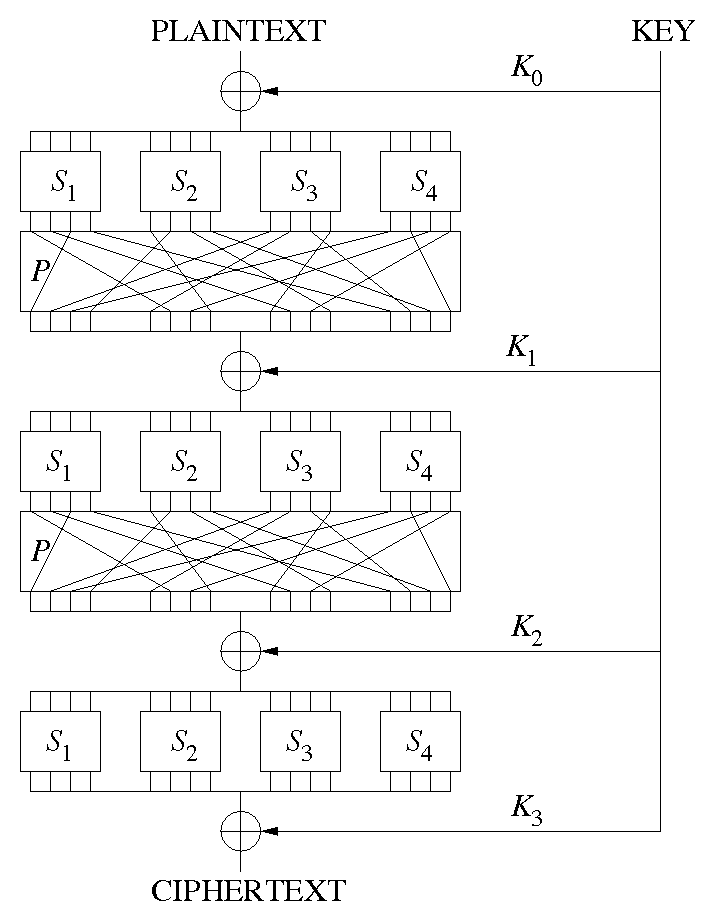
\includegraphics[scale=0.40]{spn.png} 
\caption{Substitution-Permutation Network}
\label{fig:SP}
\end{center}
\end{figure}
\end{comment}
In the next subsections we will discuss what S-boxes and P-boxes are.

\subsection{Vectorial Boolean Functions (S-boxes)}
A large part of understanding Block Ciphers, and how to attack them, will be
tied up in understanding S-boxes, (which are types of Vectorial Boolean
Functions). This section will deal with introducing and explaining them, along
with a few examples.

\begin{defn}
Any bijection $S:\{0,1\}^n \rightarrow \{0,1\}^n$ which maps boolean n-tuples
to boolean n-tuples, is called an \textbf{Substituion-box} (S-box). In this
instance, $n$ is called the block size, and we refer to an S-box with block
size $n$, as an $n$-bit S-box.
\end{defn}

What immediately follows from the fact that S is a bijection, is that
the inverse $S^{-1}$ exists, and that we can reverse the S-box.

\begin{example}
A very simple, but not very useful, S-box would be one operating on n-tuples, which just maps
every element to itself.
\begin{equation}
S_{id}: \{0,1\}^n \rightarrow \{0,1\}^n
\end{equation}
where
\begin{equation}
S_{id}(x) = x
\end{equation}

\end{example}

\begin{example}
Let's consider a simple 3 bit S-box. Since there are only 3 bits, we have 
$2^3 = 8$ possible inputs. Since S-boxes are bijections, we can only have
8 possible outputs. Thus, we can think of an S-box as a type of look-up
table.

\begin{center}
\begin{tabular}{|r|r|}
\hline
$x$ & $y = S(x)$ \\\hline
$000$ & $010$ \\\hline
$001$ & $110$ \\\hline
$010$ & $000$ \\\hline
$011$ & $100$ \\\hline
$100$ & $011$ \\\hline
$101$ & $001$ \\\hline
$110$ & $111$ \\\hline
$111$ & $101$ \\\hline
\end{tabular}
\end{center}

We can however reverse the S-box, taking $x$ to be the subject of our formula.
So instead of $y = S(x)$, we get $x = S^{-1}(y)$. Looking at the previous
table like this, we get:

\begin{center}
\begin{tabular}{|r|r|}
\hline
$y$ & $x = S^{-1}(y)$ \\\hline
$000$ & $010$ \\\hline
$001$ & $101$ \\\hline
$010$ & $000$ \\\hline
$011$ & $100$ \\\hline
$100$ & $011$ \\\hline
$101$ & $111$ \\\hline
$110$ & $000$ \\\hline
$111$ & $110$ \\\hline
\end{tabular}
\end{center}

\end{example}

\subsection{P-boxes}
S-boxes provide good confusion. What about diffusion? P-boxes.
Refer to S-box followed immediately by P-box as SP-box.

\section{Differential Properties of SP-boxes}
Next will be discussed the various differential properties of S-boxes which
allow cryptanalysts to mount an attack against a block cipher.  These include
the property that XORs do not affect differentials, as well as ways to find
relationships between input differentials and output differentials of an S-box.

\subsection{Probabilities of Differential Trails}
The previous properties discussed can be combined to give us insight into the
probabilities of differentials trails, or in plain English: Given an input
differential, how likely or probable is it that a certain output differential
occurs. This section will discuss the theory behind probabilities of
differentials. 

All of this however, is based on the assumption that these probabilities are
linearly independent. If they are not, then we can't be sure of what the
final probability is.



%%%%%%%%%%%%%%%%%%%%%%%%%%%%%%%%%%%%%%%%%%%%%%%%%%%%%%%%%%%%%%%%%%%
%                                                                 %
%                       Differential Attacks                      %
%                                                                 %
%%%%%%%%%%%%%%%%%%%%%%%%%%%%%%%%%%%%%%%%%%%%%%%%%%%%%%%%%%%%%%%%%%%


\chapter{Differential Attacks} \label{c:differential attacks}

So far we have taken a look at a number of sections, which for the most part
look fairly disjoint. In this section, we will tie these concepts together and
discuss the process whereby a differential attack can be mounted against a
block cipher. Perhaps the easiest way to do this would be by means of working
through the process on an example in various subsections.

So before we begin, we would want to clarify what assumptions need to be made
in order to mount a successful attack against the type of Block Cipher
discussed in the previous chapter.
\paragraph{}

We can reduce them to the following list:
\begin{itemize}
\item We can choose some plaintext.
\item We know or can generate the corresponding ciphertext.
\item We know the SP-boxes. 
\item We do not know the key.
\end{itemize}

Accepting those assumptions, we are ready to note down our algorithm for
attacking Block Ciphers, and specifically a SPN, with Differential
Cryptanalysis. So let's explain how we would attack an SPN then...

Firstly, for each round of our Iterated Block Cipher, we will want to search
for any pairs of inputs $(X, X')$ with XOR difference $\Delta X$, which results
in the corresponding output pair $(Y, Y')$ having XOR difference $\Delta Y$
with high probability. To be clear however in the above, $X \oplus X' =
\Delta X$ and $Y \oplus Y' = \Delta Y$. The pair $(\Delta X, \Delta Y)$ is
known as a \textbf{differential}. We can do this, since although SP-boxes affect
inputs and outputs, they do not affect differentials. This enables us to to build up a
differential characteristic for the Block Cipher. 

Thinking back to the structure of our SPN, if there is an SP-box after the last
round, we can simply invert it and get what the input would be to said SP-box,
so either way we are left facing the last round key. Then, since we know 
high-probability inputs for the last round from our differential characteristic,
we can XOR the inputs with our know ciphertext to extract the key.

In summary, once we have chosen our plaintext/ciphertext pairs, our basic
methodology for breaking the last round is as follows:
\begin{enumerate}
\item For each round up to $r-1$, compute the differentials on the SP-box.
\item Find differential characteristics with high probabilities.
\item Extract the last round key.
\end{enumerate}

We will use this strategy iteratively to break each round key, so let us
discuss each of these points in greater detail.

\section{Computing Differentials for Each Round}
So, for each round, how do we analyze an SP-box to retrieve its differentials?
Well since the SP-boxes are publicly known, we can iterate through all possible
inputs $X$ to a particular SP-box, and for each input, iterate through all
possible input differences $\Delta X$ to get input pairs $(X, X' = X \oplus
\Delta X$. Then, by sending the inputs, $X$ and $X'$ through the SP-box, we can
calculate each possible output difference $\Delta Y$ given by $\Delta Y = S(X)
\oplus S(X')$. Once we have all of these output differences, we can tally the
output differences that occur often for a given input difference, and record
them in a differential table. 

This might be best explained using an example, so let us consider the SP-box 
represented by the following table (in hexadecimal):
\begin{center}
\begin{tabular}{|r|r|}
\hline
$X$ & $S(X)$ \\\hline
0 & 3 \\\hline
1 & 5 \\\hline
2 & 2 \\\hline
3 & 1 \\\hline
4 & 6 \\\hline
5 & 7 \\\hline
6 & 4 \\\hline
7 & 0 \\\hline
8 & A \\\hline
9 & C \\\hline
A & B \\\hline
B & 8 \\\hline
C & 9 \\\hline
D & F \\\hline
E & D \\\hline
F & E \\\hline
\end{tabular}
\end{center}
You might notice that in this SP-box, function values do not seem to be particularly
well distributed. In fact, any value less than 8 is mapped to corresponding
value less than 8, and consequently values greater than or equal to 8 are mapped
to values greater than 8. In real life, this would correspond to a bad permutation
function, but we purposefully use this SP-box so that we get clear outliers in terms of
high-probabities differentials when we compute the differential table.

Thus, if we step through possible inputs, $\{0, ..., 15\}$ to our SP-box, and for
each input, XOR it with all the possible input differences $\{0, ..., 15\}$, we
get the following pairs $(X, X \oplus \Delta X)$ represented by the row and
column headings of the table below:
\begin{center}
\begin{tabular}{|c||c|c|c|c|c|c|c|c|c|c|c|c|c|c|c|c|c|}
%\multicolumn{17}{c}{$\Delta X$ values}\\
\hline
%\multirow{16}{*}{$X$}
& 0 & 1 & 2 & 3 & 4 & 5 & 6 & 7 & 8 & 9 & A & B & C & D & E & F \\\hline\hline
0 & 0 & 6 & 1 & 2 & 5 & 4 & 7 & 3 & 9 & F & 8 & B & A & C & E & D \\\hline
1 & 0 & 6 & 4 & 7 & 2 & 3 & 5 & 1 & 9 & F & D & E & A & C & B & 8 \\\hline
2 & 0 & 3 & 1 & 7 & 6 & 2 & 4 & 5 & 9 & A & 8 & E & F & C & B & D \\\hline
3 & 0 & 3 & 4 & 2 & 1 & 5 & 6 & 7 & 9 & A & D & B & F & C & E & 8 \\\hline
4 & 0 & 1 & 2 & 6 & 5 & 3 & 4 & 7 & F & 9 & B & 8 & C & A & D & E \\\hline
5 & 0 & 1 & 7 & 3 & 2 & 4 & 6 & 5 & 8 & E & 9 & A & B & D & F & C \\\hline
6 & 0 & 4 & 2 & 3 & 6 & 5 & 7 & 1 & 9 & A & D & B & F & C & E & 8 \\\hline
7 & 0 & 4 & 7 & 6 & 1 & 2 & 5 & 3 & E & D & F & 9 & 8 & B & C & A \\\hline
8 & 0 & 6 & 1 & 2 & 3 & 5 & 7 & 4 & 9 & F & 8 & B & C & D & E & A \\\hline
9 & 0 & 6 & 4 & 7 & 3 & 5 & 2 & 1 & 9 & F & D & E & B & A & C & 8 \\\hline
A & 0 & 3 & 1 & 7 & 6 & 5 & 2 & 4 & 9 & A & 8 & E & F & B & D & C \\\hline
B & 0 & 3 & 4 & 2 & 6 & 5 & 7 & 1 & 9 & A & D & B & 8 & C & F & E \\\hline
C & 0 & 6 & 4 & 7 & 3 & 5 & 2 & 1 & F & E & D & 9 & A & C & B & 8 \\\hline
D & 0 & 6 & 1 & 2 & 3 & 5 & 7 & 4 & 8 & 9 & F & B & A & C & E & D \\\hline
E & 0 & 3 & 4 & 2 & 6 & 5 & 7 & 1 & 9 & D & B & A & F & C & E & 8 \\\hline
F & 0 & 3 & 1 & 7 & 6 & 5 & 2 & 4 & E & A & 9 & 8 & F & C & B & D \\\hline
\end{tabular}
\end{center}

Each value in the above table is the $\Delta Y$ for a given $X$, the
row label, and $\Delta X$, the column label. To work out the $\Delta Y$
by hand, use the following formula:

\begin{equation}
\Delta Y = S(X) \oplus S(X \oplus \Delta X)
\end{equation}

By counting the number of times a particular output difference $\Delta Y$
occurs for a particular input difference $\Delta X$, we can generate
the following table, where the column headings are output differences
and the row headings are input differences:

\begin{center}
\begin{tabular}{|c||c|c|c|c|c|c|c|c|c|c|c|c|c|c|c|c|c|}
\hline
& 0 & 1 & 2 & 3 & 4 & 5 & 6 & 7 & 8 & 9 & A & B & C & D & E & F \\\hline\hline
0 & 16 & 0 & 0 & 0 & 0 & 0 & 0 & 0 & 0 & 0 & 0 & 0 & 0 & 0 & 0 & 0 \\\hline
1 & 0 & 2 & 0 & 6 & 2 & 0 & 6 & 0 & 0 & 0 & 0 & 0 & 0 & 0 & 0 & 0 \\\hline
2 & 0 & 6 & 2 & 0 & 6 & 0 & 0 & 2 & 0 & 0 & 0 & 0 & 0 & 0 & 0 & 0 \\\hline
3 & 0 & 0 & 6 & 2 & 0 & 0 & 2 & 6 & 0 & 0 & 0 & 0 & 0 & 0 & 0 & 0 \\\hline
4 & 0 & 2 & 2 & 4 & 0 & 2 & 6 & 0 & 0 & 0 & 0 & 0 & 0 & 0 & 0 & 0 \\\hline
5 & 0 & 0 & 2 & 2 & 2 & 10 & 0 & 0 & 0 & 0 & 0 & 0 & 0 & 0 & 0 & 0 \\\hline
6 & 0 & 0 & 4 & 0 & 2 & 2 & 2 & 6 & 0 & 0 & 0 & 0 & 0 & 0 & 0 & 0 \\\hline
7 & 0 & 6 & 0 & 2 & 4 & 2 & 0 & 2 & 0 & 0 & 0 & 0 & 0 & 0 & 0 & 0 \\\hline
8 & 0 & 0 & 0 & 0 & 0 & 0 & 0 & 0 & 2 & 10 & 0 & 0 & 0 & 0 & 2 & 2 \\\hline
9 & 0 & 0 & 0 & 0 & 0 & 0 & 0 & 0 & 0 & 2 & 6 & 0 & 0 & 2 & 2 & 4 \\\hline
A & 0 & 0 & 0 & 0 & 0 & 0 & 0 & 0 & 4 & 2 & 0 & 2 & 0 & 6 & 0 & 2 \\\hline
B & 0 & 0 & 0 & 0 & 0 & 0 & 0 & 0 & 2 & 2 & 2 & 6 & 0 & 0 & 4 & 0 \\\hline
C & 0 & 0 & 0 & 0 & 0 & 0 & 0 & 0 & 2 & 0 & 4 & 2 & 2 & 0 & 0 & 6 \\\hline
D & 0 & 0 & 0 & 0 & 0 & 0 & 0 & 0 & 0 & 0 & 2 & 2 & 10 & 2 & 0 & 0 \\\hline
E & 0 & 0 & 0 & 0 & 0 & 0 & 0 & 0 & 0 & 0 & 0 & 4 & 2 & 2 & 6 & 2 \\\hline
F & 0 & 0 & 0 & 0 & 0 & 0 & 0 & 0 & 6 & 0 & 2 & 0 & 2 & 4 & 2 & 0 \\\hline
\end{tabular}
\end{center}

Taking a look at the table above, we see that certain input differences map to
certain output differences significantly more often than others.  For example,
the input difference 5 goes to the output difference 5, 10 out of the 16 times,
giving us a probability of $\frac{10}{16}$.  For a perfect SP-box, we want each
input difference go to each output difference $\frac{1}{2^n} = \frac{1}{16}$.
Unfortunately, we know that $\Delta Y = S(X) \oplus S(X \oplus \Delta X) = S(X
\oplus \Delta X) \oplus S(X)$ so input differences map to output differences in
pairs, and thus the smallest number we could get is 2.

Up until now, we have all but ignored the effect of the key, but there is a good
reason why: the key does not affect the differentials of a round.

To see this, notice that for inputs $X$ and $X'$ and round subkey $K$, we have:
\begin{align*}
(X \oplus K) \oplus (X' \oplus K) &= X \oplus K \oplus X' \oplus K\\
&= X \oplus X' \oplus K \oplus K\\
&= X \oplus X'\\
&= \Delta X
\end{align*}

\section{Constructing a Differential Characteristic}

In the previous section, we saw how to calculate the differentials for a
particular round. However, we can conduct this process for each round, and
chain together high-probability differentials between rounds, giving us a
\textbf{differential characteristic} of the Block Cipher. We do this by using
one round's high probability output differential as the next round's input
differential.

\begin{example}
Continuing the example from the previous section, we saw that the following
input differences went to the following output differences with high
probability:
\begin{itemize}
\item $5 \rightarrow 5$ with probability $\frac{10}{16}$
\item $8 \rightarrow 9$ with probability $\frac{10}{16}$
\item $D \rightarrow C$ with probability $\frac{10}{16}$
\end{itemize}
Now suppose this was our first SP-box, with our SPN consisting of 4 rounds, we
would have the same information for each of these rounds. Perhaps the second
SP-box had a differential $9 \rightarrow 2$ with probability $\frac{8}{16}$
and the third SP-box had a differential $2 \rightarrow 6$ with probability 
$\frac{6}{16}$. Then, since these probabilities are assumed to be independent,
we can multiply them together to get a differential characteristic $8 \rightarrow
2$ with probability $\frac{10}{16} \times \frac{8}{16} \times \frac{10}{16} = 
\frac{600}{4096} = \frac{75}{512}$ for the first 3 rounds. Thus, we are assured
that plaintext pairs with a difference of 8 will result in input pairs to round
4 with a difference of 2 with high probability.
\end{example}

\begin{rem}
If the probabilities are not independent, then we can't multiply them together
and the differential attack would not work.
\end{rem}

We then use this differential charateristic in the next stage of our attack.

\section{Extracting Each Round Key}
How would we extract a key from a round? Well if we knew the input $X$ to a round,
the SP-box and the output $Y$, we could send the output back through the SP-box, to
get $S^{-1}(Y) = X \oplus K $ and XOR it with $X$ to get the key K since
\begin{equation}
S(X \oplus K) = Y.
\end{equation}

For the last round, we know what the outputs are since we can generate ciphertext
from plaintext. Unfortunately, we do not know the specific input to our last round
before the key gets mixed in. We do however know what possible plaintext input 
differences will lead to what possible input differences to round $r$ from our 
differential characteristic.

All that is then required is to choose plaintext pairs $(P, P')$ satisfying our
high-probability differential characteristic, and generate corresponding inputs
to round $r$ from the input difference to round $r$.  Now for each input pair
$(X, X')$, we can XOR the inputs $X$ and $X'$ with the inputs to our SP-box
$S^{-1}(C)$ and $S^{-1}(C')$, such that we get:

\begin{equation}
X \oplus S^{-1}(C) = K
\end{equation}
\begin{equation}
X' \oplus S^{-1}(C') = K'
\end{equation}

Thus, we get possible values for the round key $K$ and $K'$. If we have chosen
a high probability differential on which we base our input pairs, there should
be a $K$ that clearly occurs more often than others. This is then our candidate
key for that round. We then check this key against arbitrary plaintext inputs
to ensure that we get the expected ciphertext outputs, and once the key is
verified, we accept as being the correct key for the round.

Now we repeat the method for our block cipher consisting of $r-1$ rounds, and
extract each round key. Once we have all the round keys, we can easily generate
the key and we will then have broken the SPN.



%%%%%%%%%%%%%%%%%%%%%%%%%%%%%%%%%%%%%%%%%%%%%%%%%%%%%%%%%%%%%%%%%%%
%                                                                 %
%                     		Implementation                        %
%                                                                 %
%%%%%%%%%%%%%%%%%%%%%%%%%%%%%%%%%%%%%%%%%%%%%%%%%%%%%%%%%%%%%%%%%%%


\chapter{Implementation} \label{c:implementation}

In the previous chapter, statistical analysis was conducted on
SP-boxes using the following Python3 program:

\begin{verbatim}
#define an SP-box in terms list with index corresponding to input bit
first = [3,5,2,1,6,7,4,0]
second = [10,12,11,8,9,15,13,14]
sbox = first + second
size = len(sbox)
dt = []

for i in range(size):
    dt.append([0]*size)
    #print('%X & %X \\\\\\hline' % (i, sbox[i]))

def s(x):
    return sbox[x]

def outputs():
    for i in range(size):
        print(get(i))

def diffs():
    print('   ', end='')
    for i in range(size):
        print(' %X ' % i, end=' ')
    print()
    for x in range(size):
        print('%X' % x,end='| ')
        for delx in range(size):
            dely = s(x) ^ s(x^delx)
            print('%X:%X' %(delx, dely) ,end=' ')
            dt[delx][dely] += 1
        print('')
    print()

def diff_table():
    print('   ', end='')
    for i in range(size):
        print(' %X' % i, end=' ')
    print()
    for i in range(size):
        print('%X' % i,end='| ')
        for j in range(size):
            print('%2d' % dt[i][j] ,end=' ')
        print('')

diffs()
diff_table()
\end{verbatim}

%\include{py}


%%%%%%%%%%%%%%%%%%%%%%%%%%%%%%%%%%%%%%%%%%%%%%%%%%%%%%%%%%%%%%%%%%%
%                                                                 %
%                         	Conclusion 			                  %
%                                                                 %
%%%%%%%%%%%%%%%%%%%%%%%%%%%%%%%%%%%%%%%%%%%%%%%%%%%%%%%%%%%%%%%%%%%


\chapter{Conclusion} \label{c:conclusion}

In the conclusion, I will wrap up what has been discussed in my
paper, and mention what can be improved upon in the future. 

%
\chapter{LaTeX}

Note: any line that starts with ``\%'' is a comment and will be
ignored by LaTeX.

\section{Math mode}

For numbered equations (you can make the label anything you want
-- I recommend starting it with ``e'' for equation):
\begin{equation} \label{e:quadratic}
y = x^2.
\end{equation}
For unnumbered equations:
\[ y = x^2 \; \; \; \text{ for } x > 0. \]
For equation arrays:
\begin{align}
y &= (x+1)^2 \nonumber \\
  &= x^2 + 2x +1.
\end{align}
* makes it unnumbered:
\begin{align*}
y &= (x+1)^2 \nonumber \\
  &= x^2 + 2x +1.
\end{align*}


\section{Congruences etc}

Look at the next chapter, which I cut and pasted from my thesis.
If there's more stuff you don't know how to write in LaTeX just
email me about it.

\section{General notes}

The command for ``divides" is $\mid$ and the command for ``does
not divide" is $\nmid$.  To write ``is congruent'' to put $\equiv$
and for ``is not congruent to'' us $\not \equiv$.

\smallskip


\section{Style}

\emph{This is how we do italics}.

In Blum's paper \cite{Blum1}...

If you want maths in the middle of the text you put it in dollar
signs, like this: $x = 0$.

Theorems:

\begin{thm} \label{t:regular primes}

Let $(h_n)$ be an EDS and $p$ a prime not dividing $h_2$ or $h_3$.
Then there exists a positive integer $N$ such that
\[ h_n \equiv 0 \pmod p \; \; \Leftrightarrow \; \; n \equiv 0 \pmod N. \]

\end{thm}


\smallskip

This is how we do fractions:  $\frac{a}{b}$.  If you have a
fraction in a displayed equation use
\[ \dfrac{a}{b}. \]

\section{The bibliography}

I put a few references into the file ``Thyla.bib'' for you so you
could see how to do it.  Note that Rose and Blum appear in the
bibliography because they were referenced in the text, but Bach
and Shallit appears because I specifically told it to when I said
``nocite{BachandShallit}'' in the main file Thyla.tex.

\addcontentsline{toc}{chapter}{Bibliography}
\bibliographystyle{apacite}
\bibliography{bibliography}
\end{document}
